%Time-stamp: "Last modified: 2018-08-02 10:42:16 (d_yasaki)"
\documentclass[ms]{uncgdissertationexp}
\setcounter{secnumdepth}{1}
% default is 12pt, phd, doublespaced.
% Masters students should use the ma on as shown below.
% \documentclass[ma]{uncgdissertation}

%%------------------------------------------------------------------%%
%%------------------------- Import Packages ------------------------%%
%%------------------------------------------------------------------%%
%% This is where you can put other packages that you may need.
\usepackage[lofdepth,lotdepth,caption=false]{subfig}
\usepackage{fancyhdr}
\usepackage{amsmath, amssymb, graphicx}
\usepackage{xspace}
\usepackage{braket}
\usepackage{color}
\usepackage{setspace}
\usepackage{fancyvrb}
\usepackage{array}
\usepackage{ifxetex,ifluatex}
\usepackage{etoolbox}
\usepackage{booktabs}
\usepackage{xcolor}
\usepackage{tabu}
\usepackage{longtable}
\usepackage{titlesec}
\usepackage{lmodern}

\usepackage{microtype, amsfonts, amsthm}
\usepackage[colorlinks=false]{hyperref}
\pdfstringdefDisableCommands{\let\MakeUppercase\relax}
%\usepackage{showframe}
%useful package to ensure margins are correct.

% fix for pandoc 1.14
\providecommand{\tightlist}{
  \setlength{\itemsep}{0pt}\setlength{\parskip}{0pt}}

\def\tightlist{} 
%%tightlist error

%%I don't know what this does...
%\usepackage{color}
\usepackage{fancyvrb}
\newcommand{\VerbBar}{|}
\newcommand{\VERB}{\Verb[commandchars=\\\{\}]}
\DefineVerbatimEnvironment{Highlighting}{Verbatim}{commandchars=\\\{\}}
% Add ',fontsize=\small' for more characters per line
\usepackage{framed}
\definecolor{shadecolor}{RGB}{248,248,248}
\newenvironment{Shaded}{\begin{snugshade}}{\end{snugshade}}
\newcommand{\KeywordTok}[1]{\textcolor[rgb]{0.13,0.29,0.53}{\textbf{#1}}}
\newcommand{\DataTypeTok}[1]{\textcolor[rgb]{0.13,0.29,0.53}{#1}}
\newcommand{\DecValTok}[1]{\textcolor[rgb]{0.00,0.00,0.81}{#1}}
\newcommand{\BaseNTok}[1]{\textcolor[rgb]{0.00,0.00,0.81}{#1}}
\newcommand{\FloatTok}[1]{\textcolor[rgb]{0.00,0.00,0.81}{#1}}
\newcommand{\ConstantTok}[1]{\textcolor[rgb]{0.00,0.00,0.00}{#1}}
\newcommand{\CharTok}[1]{\textcolor[rgb]{0.31,0.60,0.02}{#1}}
\newcommand{\SpecialCharTok}[1]{\textcolor[rgb]{0.00,0.00,0.00}{#1}}
\newcommand{\StringTok}[1]{\textcolor[rgb]{0.31,0.60,0.02}{#1}}
\newcommand{\VerbatimStringTok}[1]{\textcolor[rgb]{0.31,0.60,0.02}{#1}}
\newcommand{\SpecialStringTok}[1]{\textcolor[rgb]{0.31,0.60,0.02}{#1}}
\newcommand{\ImportTok}[1]{#1}
\newcommand{\CommentTok}[1]{\textcolor[rgb]{0.56,0.35,0.01}{\textit{#1}}}
\newcommand{\DocumentationTok}[1]{\textcolor[rgb]{0.56,0.35,0.01}{\textbf{\textit{#1}}}}
\newcommand{\AnnotationTok}[1]{\textcolor[rgb]{0.56,0.35,0.01}{\textbf{\textit{#1}}}}
\newcommand{\CommentVarTok}[1]{\textcolor[rgb]{0.56,0.35,0.01}{\textbf{\textit{#1}}}}
\newcommand{\OtherTok}[1]{\textcolor[rgb]{0.56,0.35,0.01}{#1}}
\newcommand{\FunctionTok}[1]{\textcolor[rgb]{0.00,0.00,0.00}{#1}}
\newcommand{\VariableTok}[1]{\textcolor[rgb]{0.00,0.00,0.00}{#1}}
\newcommand{\ControlFlowTok}[1]{\textcolor[rgb]{0.13,0.29,0.53}{\textbf{#1}}}
\newcommand{\OperatorTok}[1]{\textcolor[rgb]{0.81,0.36,0.00}{\textbf{#1}}}
\newcommand{\BuiltInTok}[1]{#1}
\newcommand{\ExtensionTok}[1]{#1}
\newcommand{\PreprocessorTok}[1]{\textcolor[rgb]{0.56,0.35,0.01}{\textit{#1}}}
\newcommand{\AttributeTok}[1]{\textcolor[rgb]{0.77,0.63,0.00}{#1}}
\newcommand{\RegionMarkerTok}[1]{#1}
\newcommand{\InformationTok}[1]{\textcolor[rgb]{0.56,0.35,0.01}{\textbf{\textit{#1}}}}
\newcommand{\WarningTok}[1]{\textcolor[rgb]{0.56,0.35,0.01}{\textbf{\textit{#1}}}}
\newcommand{\AlertTok}[1]{\textcolor[rgb]{0.94,0.16,0.16}{#1}}
\newcommand{\ErrorTok}[1]{\textcolor[rgb]{0.64,0.00,0.00}{\textbf{#1}}}
\newcommand{\NormalTok}[1]{#1}
%
% commands and environments needed by pandoc snippets
% extracted from the output of `pandoc -s`
%% Make R markdown code chunks work

\ifxetex
  \usepackage{fontspec,xltxtra,xunicode}
  \defaultfontfeatures{Mapping=tex-text,Scale=MatchLowercase}
\else
  \ifluatex
    \usepackage{fontspec}
    \defaultfontfeatures{Mapping=tex-text,Scale=MatchLowercase}
  \else
    \usepackage[utf8]{inputenc}
  \fi
\fi
\DefineShortVerb[commandchars=\\\{\}]{\|}
\DefineVerbatimEnvironment{Highlighting}{Verbatim}{commandchars=\\\{\}}
% Add ',fontsize=\small' for more characters per line



%%------------------------------------------------------------------%%
%%--------------------------- Content ------------------------------%%
%%------------------------------------------------------------------%%
%% Members of committee.  Guidelines say don't use Dr.
%% Masters students are required to have chair plus two
%% PhD students require chair plus three.
%% The class can handle up to chair plus five.
\chair{Parke Rublee}
\member{Anne Hershey}
\member{Martin Tsui}
%%\member{}

%% Your name goes here.
%% \student{Firstname}{Lastname}
%% Some other options
%%\student{Joe Michael}{Schmoe}  % a full middle name
\student{Ashley S.}{Williams}       % a middle initial

%% Thesis Title
%%    +  Capitalize first letter of important words.
%%    +  Use inverted pyramid shape if title spans more than one line.
%%  Note: You can force break the title onto multiple lines using
%%  \break instead of \\.
\title{Response of Mercury Methylating Bacteria to the Dan River Coal Ash Spill
with a Survey of Metal Tolerance of Microorganisms Associated with Coal
Ash}

%% Degree year.
\degreeyear{2019}


%%------------------------------------------------------------------%%
%%----------------------- Personal Macros --------------------------%%
%%------------------------------------------------------------------%%
%% A central location to add your favorite macros.  A few examples are
%% given below.  See tips for samples.

%% In order to get singlespacing, uncomment the line below.
%\renewcommand{\doublespacing}{\singlespacing}

%% Theorem, Lemma, etc. environments.  You can rename if you wish.
% Theorem style and numbering convention
\theoremstyle{plain}
\newtheorem{theorem}{Theorem}[chapter]
\newtheorem{lemma}[theorem]{Lemma}
\newtheorem{proposition}[theorem]{Proposition}
\newtheorem{conjecture}[theorem]{Conjecture}
\newtheorem{corollary}[theorem]{Corollary}
\newtheorem{algorithm}[theorem]{Algorithm}

% Definition type object style and numbering convention
\theoremstyle{definition}
\newtheorem{definition}[theorem]{Definition}
\newtheorem{example}[theorem]{Example}

% Remark type object style and numbering
\theoremstyle{remark}
\newtheorem*{remark}{Remark}  % the star makes them not numbered
\newtheorem*{notation}{Notation}
\newcommand{\titlecaption}[2]{\caption[#1]{#1. #2}}

%% Other macros
\newcommand{\ZZ}{\mathbb{Z}}  % Integers
\newcommand{\XX}{\mathfrak{X}}

%\bibliography{references}

%%------------------------------------------------------------------%%
\begin{document}
\frontmatter      % required

%%------------------------------------------------------------------%%
%% -------------------------- Abstract -----------------------------%%
%%------------------------------------------------------------------%%
\begin{abstract}
  This is my abstract. The abstract page is a required component of the
  thesis/dissertation. The abstract should be a brief summary of the
  paper, stating only the problem, procedures used, and the most
  significant results and conclusions. Explanations and opinions are
  omitted. Remember to include the necessary information regarding any
  multimedia components included in the document. The abstract must be
  approved by your advisor/committee chair.
\end{abstract}
%%------------------------------------------------------------------%%
%%---------------------------- Title page --------------------------%%
%%------------------------------------------------------------------%%
%% The title page is required.
\maketitlepage

%%------------------------------------------------------------------%%
%% ------------------------ Copyright page -------------------------%%
%%------------------------------------------------------------------%%
%% This page is required if you opt for a copyright.  Otherwise, don't
% include it.  To omit, just comment out the line below.
%\makecopyrightpage

%%------------------------------------------------------------------%%
%%---------------------------- Dedication --------------------------%%
%%------------------------------------------------------------------%%
\begin{dedication}
  The dedication is often short. Longer statements are usually in the
  acknowledgements. The dedication is optional.
\end{dedication}
%%------------------------------------------------------------------%%
%%------------------------ Approval page  --------------------------%%
%%------------------------------------------------------------------%%
%% The approval page is required.  If all of your infomation is entered
%% correctly in the contents section, this should come out correctly.
\makeapprovalpage

%%------------------------------------------------------------------%%
%%-------------------------- Acknowledgements ----------------------%%
%%------------------------------------------------------------------%%
%% The acknowledgements are optional but highly recommended.  See tips
%% for details.
\begin{acknowledgments}
  It is customary to recognize the assistance of the advisor and/or
  committee chair, all other members of the committee, and only those
  organizations and/or persons who actually aided the research. If
  financial support was provided to make the study possible, credit for
  such assistance should be given.
\end{acknowledgments}
%%------------------------------------------------------------------%%
%%----------------------------- Preface ----------------------------%%
%%------------------------------------------------------------------%%
%% The preface is optional.
%%\begin{preface}
%%A preface is a statement that either explains the author's
%%reasons for pursuing this subject matter or provides a personal
%%comment about the subject that would not otherwise be included in
%%the document.
%%\end{preface}


%%------------------------------------------------------------------%%
%%---------------------- Table of Contents -------------------------%%
%%------------------------------------------------------------------%%
%% The table of contents is required.
\tableofcontents

%%------------------------------------------------------------------%%
%%---------------------- List of Tables ----------------------------%%
%%------------------------------------------------------------------%%
% Recommended if you have tables.  Comment out if you don't have
% tables.

  \listoftables
  

%%------------------------------------------------------------------%%
%%---------------------- List of Figures ---------------------------%%
%%------------------------------------------------------------------%%
% Recommended if you have figures.  Comment out if you don't have
% figures.

  \listoffigures
  

%%------------------------------------------------------------------%%
%% This signifies that you are done with the frontmatter and ready to
%% proceed to the main part.  The rest of your document goes below.
\mainmatter % required
%%------------------------------------------------------------------%%
 
  \chapter{Introduction}\label{intro}
  
  Coal is the second most used fuel for electricity generation in the
  United States. In 2017, approximately 30\% of all electricity production
  was fueled by coal combustion (Administration, 2019). Although the
  percentage has fallen in recent years due to retirement of plants and
  increase in natural gas and other energy sources, coal remains a main
  fuel for electricity. During the process of coal combustion, coal
  combustion residuals, or coal ash, is produced.
  
  Coal combustion residues (CCRs) include fly ash, bottom ash, and flue
  gas desulfurized gypsum. Fly ash is a fine powdery substance, comprised
  primarily of silica that moves up the exhaust system. It is produced
  during the combustion of finely ground coal and most is captured from
  the exhaust using electrostatics and scrubber systems (US EPA, 2014a).
  Bottom ash is formed during the combustion of pulverized coal in
  boilers. It ranges in size from fine sand to fine gravel and is grey to
  black in color. Bottom ash is too large to be carried up the exhaust
  system and is collected in an ash hopper (US EPA, 2014b). Flue gas
  desulfurized gypsum is not a direct product of coal combustion, but a
  product of the scrubber system to remove SO2 emissions from exhaust (US
  EPA, 2014c).
  
  Physical and chemical properties of coal ash are determined by the
  geographical location where the raw coal was mined, the type of boiler,
  and the operating conditions of the power plant (Jayaranjan et al.,
  2014). Fly ash is composed mainly of oxides such as \(\mathrm{SiO_2}\),
  \(\mathrm{Al_2O}\), \(\mathrm{Fe_2O}\), \(\mathrm{TiO_2}\), and
  \(\mathrm{CaO}\). All natural elements can be found in coal ash, trace
  elements include, As, Cd, Cr, Hg, Pb, Se, and Zn (Greely Jr. et al.,
  2014; Jayaranjan et al., 2014; Shaheen et al., 2014). Coal bottom ash
  consists of silicate, carbonate, aluminate, ferrous materials and
  several of heavy metals and metalloids. Like fly ash, the chemical
  composition of the bottom ash is dependent on the source of the raw
  coal, boiler type, and the refinement process of the raw coal
  (Jayaranjan et al., 2014).
  
  Once produced and collected, CCRs are transported to an impoundment pond
  or landfill. Impoundment ponds are constructed either lined or unlined;
  open to the atmosphere or capped. In an open lagoon, the waste settles
  to the bottom of the pond, leaving the shallow surface water free of
  waste. To prevent overflow of these ponds, this shallow water is pumped
  and directed to a waterway adjacent to the power plant. In the US, of
  the approximately 120 Mt of CCRs are produced annually, 54\% is disposed
  of in landfills or surface impoundments (American Coal Ash Association,
  2012). Leaching and impoundment failures allow the mobilization of CCRs
  including their associated heavy metals into the environment, where
  these metals may enter the food web directly or indirectly through
  microbially-mediated transformations (Cabral et al., 2016; Deonarine et
  al., 2013; Otter et al., 2012).
  
  \chapter{RESPONSE OF MERCURY METHYLATING BACTERIA TO THE COAL ASH SPILL
  IN THE DAN RIVER}\label{pcr}
  
  \section{Abstract}\label{abstract}
  
  \section{Introduction}\label{introduction}
  
  On February, 2, 2014, two storm water drainage pipes located under a
  coal ash impoundment pond at the Duke Energy Dan River Steam Station
  near Eden, NC collapsed, releasing approximately 28,000 cubic yards of
  coal ash and about 27 million gallons of untreated ash wastewater into
  the Dan River (Dennis Lemly, 2015). Following the spill, water and
  sediment was sampled from the river and Kerr Reservoir downstream of the
  spill to determine water quality and human health concerns. Test results
  show no constituents to be at levels exceeding safe limits in the water
  column (US EPA, 2014d). Duke Energy dredged ash deposits at two
  locations along the river, but likely over 90\% of the ash remains
  buried in river sediments or has been deposited into Kerr Lake (NC DEQ,
  2014). While the test results are encouraging for immediate water
  quality, the long-term concern is the effect of mobilization of coal ash
  constituents into the riverine food webs.
  
  One constituent of particular concern during leaching and/or impoundment
  failure is mercury. Mercury, a known neurotoxin and potential endocrine
  disruptor has a high affinity for sulfhydryl groups in proteins where
  destabilization leads to decreased enzymatic activity and reduced
  overall fitness (Driscoll et al., 2013; Ehrlich and Newman, 2008). In
  submerged anoxic sediments under certain conditions, inorganic mercury
  (\(\mathrm{Hg^{2+}}\)) can be converted into MeHg by microbial
  metabolism (Dash and Das, 2014; Schaefer et al., 2011). Methylmercury
  (MeHg) bioaccumulates and biomagnifies in the river food webs, posing a
  health risk to local residents who consume fish. (Dash and Das, 2014;
  Otter et al., 2012; Rowe, 2014). The total available amount of MeHg
  within an ecosystem is controlled by multiple microbial and abiotic
  processes that reduce availability of \(\mathrm{Hg^{2+}}\) or
  degradation of MeHg. \(\mathrm{Hg^{2+}}\) can be volatilized as
  \(\mathrm{Hg^{0}}\) through photoreduction or by bacteria with the merA
  gene (Boyd and Barkay, 2012). Additionally, MeHg can be demethylated
  into \(\mathrm{Hg^{2+}}\) by sunlight (Tsui et al., 2013) or microbes
  with the merB gene (Bizily et al., 1999).
  
  Microorganisms have developed various mechanisms to mitigate effects of
  high concentrations of heavy metal toxins. These include reduction of
  the metal to a less toxic form, metal complexation, efflux pumps via an
  energy-dependent membrane transporter, and extracellular sequestration
  (Binkley and Simpson, 2003; Poulain and Barkay, 2013). MeHg is produced
  in anaerobic conditions predominately by sulfate reducing bacteria (SRB)
  iron reducing bacteria (IRB) and methanogens (Liu et al., 2014). Coal
  ash may provide the necessary substrates such as sulfates to stimulate
  the microbial methylation of Hg (Deonarine et al., 2013).
  
  Two genes are required for methylation of Hg, hgcA and hgcB. As
  \(\mathrm{Hg^{2+}}\) enters the cell, a methylated-HgcA protein
  transfers a CH3 group to \(\mathrm{Hg^{2+}}\) within the cytosol. HgcB
  protein is then required to recycle the methylated-HgcA protein (Poulain
  and Barkay, 2013). The hgcAB sequence is conserved across multiple
  genera and therefore could be utilized as a molecular biomarker for
  suspected contaminated sites with real-time quantitative PCR
  (Christensen et al., 2016; Dash and Das, 2014; Lima de Silva et al.,
  2012; Parks et al., 2009). Liu et al. (2014) found that the hgcA
  abundance and the concentration of MeHg in rice paddy soil near the
  Wanshan Hg mining area was positively correlated (Liu et al., 2014).
  This finding suggests that microbes may be contributing to the MeHg in
  the sampled soils. They also found high genetic diversity within the
  microbial community and that environmental factors such as total Hg,
  \(\mathrm{SO_4}\), \(\mathrm{NH_4}\), and organic matter influenced the
  community structure. After phylogenetic analysis, the representative
  taxa in the community consisted of Deltaproteobacteria, Firmicutes,
  Chloroflexi, Euryarchaeota, and two novel taxa (Liu et al., 2014).
  
  In 2008 a dike failure at the Tennessee Valley Authority Kingston Fossil
  Plant coal ash pond in Harriman, Tennessee, released an estimated 5.4
  million cubic yards of ash into the surrounding community and rivers
  (Ruhl et al., 2010). The release ruptured a natural gas line, disrupted
  power and transportation, destroyed three homes, and resulted in the
  evacuation of nearby neighborhoods. The impoundment pond has since been
  rebuilt and reinforced to resist natural disasters such as earthquakes
  (TVA, 2011). In sediment samples collected downstream following the
  spill, total mercury concentrations were three to four times greater
  than sediments upstream of the spill. MeHg was also slightly higher than
  upstream (Deonarine et al., 2013).
  
  The coal ash spill into the Dan River has mobilized heavy metals into
  the environment. The extent of long-term effects of methylated mercury
  into the food chain in the river is unknown. Mercury, along with other
  coal ash constituents may stimulate mercury-methylating microorganisms
  in anaerobic sediments. The goal of this study is to determine the
  overall microbial community response and specifically hgcA abundance as
  a result of the Dan River coal ash spill.
  
  \subsection{Objective and hypothesis:}\label{objective-and-hypothesis}
  
  Determine spatial distribution of mercury-methylating taxa as a result
  of the coal ash spill using qPCR. I hypothesize that there will be
  increased abundance of the hgcA genes and therefore, mercury methylating
  taxa downstream of spill site due to stimulation of sulfate and iron
  reducing bacteria and methanogens by coal ash constituents present in
  the sediment.
  
  \section{Methods}\label{methods}
  
  \subsection{Study Sites and Sediment
  Collection}\label{study-sites-and-sediment-collection}
  
  The Dan River is a 344 km river that rises in Patrick Co. Virginia and
  crosses into North Carolina in Stokes County. It flows across the border
  between NC and VA several times before flowing into the Kerr Reservoir
  on the Roanoke River which then flows to the Atlantic Ocean at the
  Albemarle Sound in North Carolina. This study encompasses sites upstream
  of the spill site in Eden, NC and downstream to Milton, NC, a 103 km
  section of the Dan.
  
  To characterize the extent of the coal ash spill impact on the microbial
  community, samples were collected at three upstream reference sites, one
  site parallel to the ash ponds but upstream of the spill (leaching
  site), and five downstream sites including near two sites that were
  dredged for remediation, one at Town Creek, near the spill site and one
  near Abreu-Grogan Park, Danville, Va., and depositional sites that were
  not dredged near Danville (Figure \ref{fig:map}).
  \begin{Shaded}
  \begin{Highlighting}[]
  \NormalTok{knitr}\OperatorTok{::}\KeywordTok{include_graphics}\NormalTok{(}\DataTypeTok{path =} \StringTok{"figure/map.png"}\NormalTok{)}
  \end{Highlighting}
  \end{Shaded}
  \begin{figure}
  
  {\centering 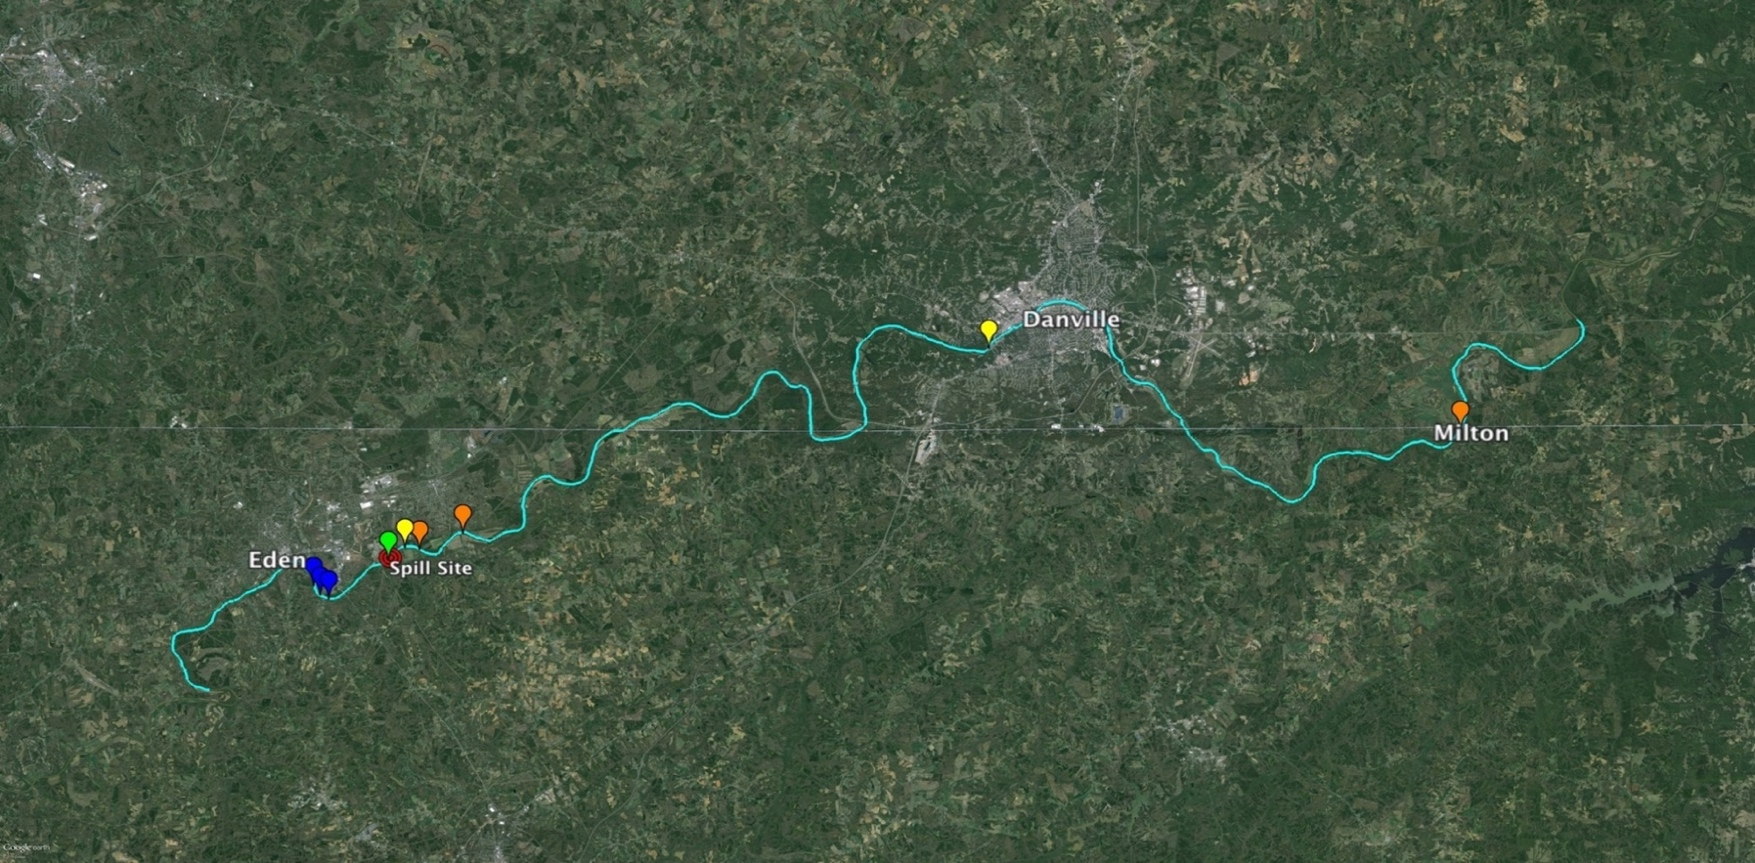
\includegraphics[width=400pt]{figure/map} 
  
  }
  
  \caption{Map}\label{fig:map}
  \end{figure}
  Each site was accessed by motorboat, where sediment from the riverbank
  and channel was collected. Riverbank sediment cores were collected in
  triplicate using a piston-stule coring device. Channel samples were
  collected using a small dredge. Sediment cores were segmented by depth
  and mixed according to one of three sampling schemes to reduce the total
  number of samples to be assayed. 0.25 \(\mathrm{cm^3}\) samples were
  preserved in CTAB (cetyltrimethylammonium bromide) for DNA extraction.
  Channel sediment was mixed thoroughly then 0.25 \(\mathrm{cm^3}\) was
  preserved in CTAB.
  
  Sampling Scheme:
  \begin{enumerate}
  \def\labelenumi{\Alph{enumi}.}
  \item
    Sediment cores extracted in triplicate, each 0-8 cm and 8-16 cm
    segments sampled
  \item
    Triplicate sediment cores pooled at 0-2 cm, 10-12 cm, 15-17 cm
  \item
    Triplicate sediment cores pooled 0-8 cm and 8-16 cm segments sampled.
  \end{enumerate}
  \subsection{DNA extraction and qPCR}\label{dna-extraction-and-qpcr}
  
  A CTAB extraction was performed using standard protocol for each sample
  (Stewart and Via 1993). The DNA extracted was quantified and
  subsequently diluted to a standard concentration of 5 ng/L and stored in
  a 4C refrigerator. Extracted DNA quantity and purity were determined
  from 2 μl subsamples of each extraction using Thermo Scientific Nanodrop
  Spectrophotometer based on the 260/280 wavelength ratio.
  
  An Applied Biosystems StepOne\^{}TM real-time PCR System was utilized to
  detect, amplify, and quantify target DNA gene proxies and representative
  taxa to meet the Objective. Primers were chosen from the literature
  based on targeting a general metabolic category. These include generic
  primers to the hgcA gene, a sulfate reducing gene, dsr, the 16S rDNA of
  iron reducing bacteria, and methanogens (Geets et al. 2008, Schaefer et
  al. 2013, Wagner et al.1998, Wright and Primm 2003, Table X). This
  approach will define the microbial community abundance encompassed
  within each sample. Each reaction contained the following: 10µL of Power
  Sybr® Green PCR master mix, 1µL of forward primer, 1µL of reverse
  primer, 8µL of sterile deionized water, and 1µL of extracted DNA. Three
  negative control reactions, samples repeated in triplicate, and positive
  standard controls serially diluted in triplicate, were ran in each 48
  well plate. The relative abundance of targets were computed by the
  StepOne software using the generated standard curve. The melt curve was
  examined to manually ensure that none of the amplifications were due to
  a false positive. Statistical analyses including one and two-way ANOVA
  and regression analyses were performed to determine if a significant
  difference exists between amounts of targeted DNA collected from sites
  upstream versus downstream of spill site and within depths of core
  samples.
  
  \subsection{Statistical Analysis}\label{statistical-analysis}
  
  \section{Results}\label{results}
  
  \section{Discussion}\label{discussion}
  
  \chapter{IDENTIFICATION AND CHARACTERIZATION OF HEAVY METAL TOLERANCE OF
  BACTERIA CULTURED FROM COAL ASH}\label{math-sci}
  
  \section*{Math}\label{Math}
  \addcontentsline{toc}{section}{Math}
  
  \TeX~is the best way to typeset mathematics. Donald Knuth designed
  \TeX~when he got frustrated at how long it was taking the typesetters to
  finish his book, which contained a lot of mathematics. One nice feature
  of \emph{R Markdown} is its ability to read LaTeX code directly.
  
  If you are doing a thesis that will involve lots of math, you will want
  to read the following section which has been commented out. If you're
  not going to use math, skip over or delete this next commented section.
  
  MATH and PHYSICS majors: Uncomment the following section
  --\textgreater{}
  
  \[\sum_{j=1}^n (\delta\theta_j)^2 \leq {{\beta_i^2}\over{\delta_i^2 + \rho_i^2}}
  \left[ 2\rho_i^2 + {\delta_i^2\beta_i^2\over{\delta_i^2 + \rho_i^2}} \right] \equiv \omega_i^2
  \]
  
  From Informational Dynamics, we have the following (Dave Braden):
  
  After \emph{n} such encounters the posterior density for \(\theta\) is
  
  \[
  \pi(\theta\vert X_1< y_1,\dots,X_n<y_n) \varpropto \pi(\theta) \prod_{i=1}^n\int_{-\infty}^{y_i}
     \exp\left(-{(x-\theta)^2\over{2\sigma^2}}\right)\ dx
  \]
  
  Another equation:
  
  Lapidus and Pindar, Numerical Solution of Partial Differential Equations
  in Science and Engineering. Page 54
  
  \[
  \int_t\left\{\sum_{j=1}^3 T_j \left({d\phi_j\over dt}+k\phi_j\right)-kT_e\right\}w_i(t)\ dt=0,
     \qquad\quad i=1,2,3.
  \]
  
  L\&P Galerkin method weighting functions. Page 55
  
  \[
  \sum_{j=1}^3 T_j\int_0^1\left\{{d\phi_j\over dt} + k\phi_j\right\} \phi_i\ dt
     = \int_{0}^1k\,T_e\phi_idt, \qquad i=1,2,3 \]
  
  Another L\&P (p145)
  
  \[
  \int_{-1}^1\!\int_{-1}^1\!\int_{-1}^1 f\big(\xi,\eta,\zeta\big)
     = \sum_{k=1}^n\sum_{j=1}^n\sum_{i=1}^n w_i w_j w_k f\big( \xi,\eta,\zeta\big).
  \]
  
  Another L\&P (p126)
  
  \[
  \int_{A_e} (\,\cdot\,) dx dy = \int_{-1}^1\!\int_{-1}^1 (\,\cdot\,) \det[J] d\xi d\eta.
  \] --\textgreater{}
  
  \section{Chemistry 101: Symbols \{-\#\}}\label{chemistry-101-symbols--}
  
  Chemical formulas will look best if they are not italicized. Get around
  math mode's automatic italicizing in LaTeX by using the argument
  \texttt{\$\textbackslash{}mathrm\{formula\ here\}\$}, with your formula
  inside the curly brackets. (Notice the use of the backticks here which
  enclose text that acts as code.)
  
  So, \(\mathrm{Fe_2^{2+}Cr_2O_4}\) is written
  \texttt{\$\textbackslash{}mathrm\{Fe\_2\^{}\{2+\}Cr\_2O\_4\}\$}.
  
  \noindent Exponent or Superscript: \(\mathrm{O^-}\)
  
  \noindent Subscript: \(\mathrm{CH_4}\)
  
  To stack numbers or letters as in \(\mathrm{Fe_2^{2+}}\), the subscript
  is defined first, and then the superscript is defined.
  
  \noindent Bullet: CuCl \(\bullet\) \(\mathrm{7H_{2}O}\)
  
  \noindent Delta: \(\Delta\)
  
  \noindent Reaction Arrows: \(\longrightarrow\) or
  \(\xrightarrow{solution}\)
  
  \noindent Resonance Arrows: \(\leftrightarrow\)
  
  \noindent Reversible Reaction Arrows: \(\rightleftharpoons\)
  
  \subsection{Typesetting reactions}\label{typesetting-reactions}
  
  You may wish to put your reaction in an equation environment, which
  means that LaTeX will place the reaction where it fits and will number
  the equations for you.
  \begin{equation}
    \mathrm{C_6H_{12}O_6  + 6O_2} \longrightarrow \mathrm{6CO_2 + 6H_2O}
    \label{eq:reaction}
  \end{equation}
  We can reference this combustion of glucose reaction via Equation
  \eqref{eq:reaction}.
  
  \subsection{Other examples of
  reactions}\label{other-examples-of-reactions}
  
  \(\mathrm{NH_4Cl_{(s)}}\) \(\rightleftharpoons\)
  \(\mathrm{NH_{3(g)}+HCl_{(g)}}\)
  
  \noindent \(\mathrm{MeCH_2Br + Mg}\) \(\xrightarrow[below]{above}\)
  \(\mathrm{MeCH_2\bullet Mg \bullet Br}\)
  
  \section{Physics}\label{physics}
  
  Many of the symbols you will need can be found on the math page
  \url{http://web.reed.edu/cis/help/latex/math.html} and the Comprehensive
  LaTeX Symbol Guide
  (\url{http://mirror.utexas.edu/ctan/info/symbols/comprehensive/symbols-letter.pdf}).
  
  \section{Biology}\label{biology}
  
  You will probably find the resources at
  \url{http://www.lecb.ncifcrf.gov/~toms/latex.html} helpful, particularly
  the links to bsts for various journals. You may also be interested in
  TeXShade for nucleotide typesetting
  (\url{http://homepages.uni-tuebingen.de/beitz/txe.html}). Be sure to
  read the proceeding chapter on graphics and tables.
  
  \chapter{Tables, Graphics, References, and Labels}\label{ref-labels}
  
  \section{Tables}\label{tables}
  
  By far the easiest way to present tables in your thesis is to store the
  contents of the table in a CSV or Excel file, then read that file in to
  your R Markdown document as a data frame. Then you can style the table
  with the \texttt{kable} function, or functions in the
  \href{https://cran.r-project.org/web/packages/kableExtra/index.html}{kableExtra}
  pacakge.
  
  In addition to the tables that can be automatically generated from a
  data frame in \textbf{R} that you saw in {[}R Markdown Basics{]} using
  the \texttt{kable} function, you can also create tables using
  \emph{pandoc}. (More information is available at
  \url{http://pandoc.org/README.html\#tables}.) This might be useful if
  you don't have values specifically stored in \textbf{R}, but you'd like
  to display them in table form. Below is an example. Pay careful
  attention to the alignment in the table and hyphens to create the rows
  and columns. Generally I don't recommend this approach of typing the
  table directly into your R Markdown document.
  \begin{longtable}[]{@{}ccc@{}}
  \caption{\label{tab:inher} Correlation of Inheritance Factors for Parents
  and Child}\tabularnewline
  \toprule
  \begin{minipage}[b]{0.29\columnwidth}\centering\strut
  Factors\strut
  \end{minipage} & \begin{minipage}[b]{0.47\columnwidth}\centering\strut
  Correlation between Parents \& Child\strut
  \end{minipage} & \begin{minipage}[b]{0.16\columnwidth}\centering\strut
  Inherited\strut
  \end{minipage}\tabularnewline
  \midrule
  \endfirsthead
  \toprule
  \begin{minipage}[b]{0.29\columnwidth}\centering\strut
  Factors\strut
  \end{minipage} & \begin{minipage}[b]{0.47\columnwidth}\centering\strut
  Correlation between Parents \& Child\strut
  \end{minipage} & \begin{minipage}[b]{0.16\columnwidth}\centering\strut
  Inherited\strut
  \end{minipage}\tabularnewline
  \midrule
  \endhead
  \begin{minipage}[t]{0.29\columnwidth}\centering\strut
  Education\strut
  \end{minipage} & \begin{minipage}[t]{0.47\columnwidth}\centering\strut
  -0.49\strut
  \end{minipage} & \begin{minipage}[t]{0.16\columnwidth}\centering\strut
  Yes\strut
  \end{minipage}\tabularnewline
  \begin{minipage}[t]{0.29\columnwidth}\centering\strut
  Socio-Economic Status\strut
  \end{minipage} & \begin{minipage}[t]{0.47\columnwidth}\centering\strut
  0.28\strut
  \end{minipage} & \begin{minipage}[t]{0.16\columnwidth}\centering\strut
  Slight\strut
  \end{minipage}\tabularnewline
  \begin{minipage}[t]{0.29\columnwidth}\centering\strut
  Income\strut
  \end{minipage} & \begin{minipage}[t]{0.47\columnwidth}\centering\strut
  0.08\strut
  \end{minipage} & \begin{minipage}[t]{0.16\columnwidth}\centering\strut
  No\strut
  \end{minipage}\tabularnewline
  \begin{minipage}[t]{0.29\columnwidth}\centering\strut
  Family Size\strut
  \end{minipage} & \begin{minipage}[t]{0.47\columnwidth}\centering\strut
  0.18\strut
  \end{minipage} & \begin{minipage}[t]{0.16\columnwidth}\centering\strut
  Slight\strut
  \end{minipage}\tabularnewline
  \begin{minipage}[t]{0.29\columnwidth}\centering\strut
  Occupational Prestige\strut
  \end{minipage} & \begin{minipage}[t]{0.47\columnwidth}\centering\strut
  0.21\strut
  \end{minipage} & \begin{minipage}[t]{0.16\columnwidth}\centering\strut
  Slight\strut
  \end{minipage}\tabularnewline
  \bottomrule
  \end{longtable}
  We can also create a link to the table by doing the following: Table
  \ref{tab:inher}. If you go back to {[}Loading and exploring data{]} and
  look at the \texttt{kable} table, we can create a reference to this max
  delays table too: Table \ref{tab:maxdelays}. The addition of the
  \texttt{(\textbackslash{}\#tab:inher)} option to the end of the table
  caption allows us to then make a reference to Table
  \texttt{\textbackslash{}@ref(tab:label)}. Note that this reference could
  appear anywhere throughout the document after the table has appeared.
  
  \clearpage
  
  \section{Figures}\label{figures}
  
  If your thesis has a lot of figures, \emph{R Markdown} might behave
  better for you than that other word processor. One perk is that it will
  automatically number the figures accordingly in each chapter. You'll
  also be able to create a label for each figure, add a caption, and then
  reference the figure in a way similar to what we saw with tables
  earlier. If you label your figures, you can move the figures around and
  \emph{R Markdown} will automatically adjust the numbering for you. No
  need for you to remember! So that you don't have to get too far into
  LaTeX to do this, a couple \textbf{R} functions have been created for
  you to assist. You'll see their use below.
  
  In the \textbf{R} chunk below, we will load in a picture stored as
  \texttt{uw.png} in our main directory. We then give it the caption of
  ``UW logo'', the label of ``uwlogo'', and specify that this is a figure.
  Make note of the different \textbf{R} chunk options that are given in
  the R Markdown file (not shown in the knitted document).
  \begin{Shaded}
  \begin{Highlighting}[]
  \NormalTok{knitr}\OperatorTok{::}\KeywordTok{include_graphics}\NormalTok{(}\DataTypeTok{path =} \StringTok{"figure/uw.png"}\NormalTok{)}
  \end{Highlighting}
  \end{Shaded}
  \begin{figure}
  
\includegraphics[width=6.25in]{figure/uw} \caption{UW logo}\label{fig:uwlogo}
  \end{figure}
  Here is a reference to the UW logo: Figure \ref{fig:uwlogo}. Note the
  use of the \texttt{fig:} code here. By naming the \textbf{R} chunk that
  contains the figure, we can then reference that figure later as done in
  the first sentence here. We can also specify the caption for the figure
  via the R chunk option \texttt{fig.cap}.
  
  \clearpage 
  
  Below we will investigate how to save the output of an \textbf{R} plot
  and label it in a way similar to that done above. Recall the
  \texttt{flights} dataset from Chapter \ref{rmd-basics}. (Note that we've
  shown a different way to reference a section or chapter here.) We will
  next explore a bar graph with the mean flight departure delays by
  airline from Portland for 2014. Note also the use of the \texttt{scale}
  parameter which is discussed on the next page.
  \begin{Shaded}
  \begin{Highlighting}[]
  \NormalTok{flights }\OperatorTok\StringTok{ }\KeywordTok{group_by}\NormalTok{(carrier) }\OperatorTok
  \StringTok{  }\KeywordTok{summarize}\NormalTok{(}\DataTypeTok{mean_dep_delay =} \KeywordTok{mean}\NormalTok{(dep_delay)) }\OperatorTok
  \StringTok{  }\KeywordTok{ggplot}\NormalTok{(}\KeywordTok{aes}\NormalTok{(}\DataTypeTok{x =}\NormalTok{ carrier, }\DataTypeTok{y =}\NormalTok{ mean_dep_delay)) }\OperatorTok{+}
  \StringTok{  }\KeywordTok{geom_bar}\NormalTok{(}\DataTypeTok{position =} \StringTok{"identity"}\NormalTok{, }\DataTypeTok{stat =} \StringTok{"identity"}\NormalTok{, }\DataTypeTok{fill =} \StringTok{"red"}\NormalTok{)}
  \end{Highlighting}
  \end{Shaded}
  \begin{figure}
  \centering
  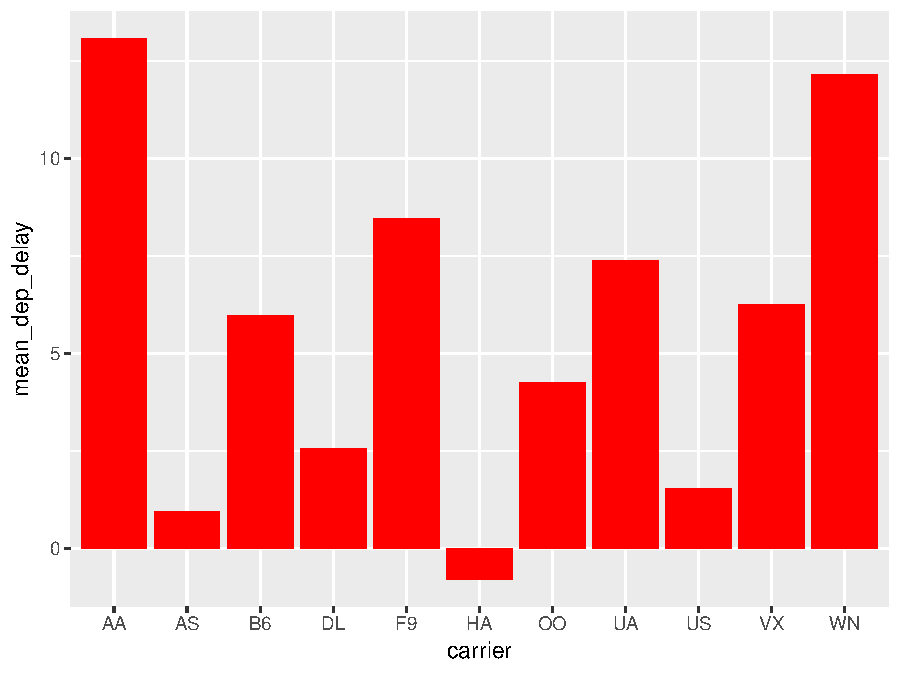
\includegraphics{thesis_files/figure-latex/delaysboxplot-1.pdf}
  \caption{\label{fig:delaysboxplot}Mean Delays by Airline}
  \end{figure}
  Here is a reference to this image: Figure \ref{fig:delaysboxplot}.
  
  A table linking these carrier codes to airline names is available at
  \url{https://github.com/ismayc/pnwflights14/blob/master/data/airlines.csv}.
  
  \clearpage
  
  \section{Footnotes and Endnotes}\label{footnotes-and-endnotes}
  
  You might want to footnote something.\footnote{footnote text} The
  footnote will be in a smaller font and placed appropriately. Endnotes
  work in much the same way.
  
  \section{Bibliographies}\label{bibliographies}
  
  Of course you will need to cite things, and you will probably accumulate
  an armful of sources. There are a variety of tools available for
  creating a bibliography database (stored with the .bib extension). In
  addition to BibTeX suggested below, you may want to consider using the
  free and easy-to-use tool called Zotero. Some Zotero documentation is at
  \url{http://libguides.reed.edu/citation/zotero}. In addition, a tutorial
  is available from Middlebury College at
  \url{http://sites.middlebury.edu/zoteromiddlebury/}.
  
  \emph{R Markdown} uses \emph{pandoc} (\url{http://pandoc.org/}) to build
  its bibliographies. One nice caveat of this is that you won't have to do
  a second compile to load in references as standard LaTeX requires. To
  cite references in your thesis (after creating your bibliography
  database), place the reference name inside square brackets and precede
  it by the ``at'' symbol. For example, here's a reference to a book about
  worrying: ({\textbf{???}}). This \texttt{Molina1994} entry appears in a
  file called \texttt{thesis.bib} in the \texttt{bib} folder. This
  bibliography database file was created by a program called BibTeX. You
  can call this file something else if you like (look at the YAML header
  in the main .Rmd file) and, by default, is to placed in the \texttt{bib}
  folder.
  
  For more information about BibTeX and bibliographies, see
  (\url{http://web.reed.edu/cis/help/latex/index.html})\footnote{({\textbf{???}})}.
  There are three pages on this topic: \emph{bibtex} (which talks about
  using BibTeX, at \url{http://web.reed.edu/cis/help/latex/bibtex.html}),
  \emph{bibtexstyles} (about how to find and use the bibliography style
  that best suits your needs, at
  \url{http://web.reed.edu/cis/help/latex/bibtexstyles.html}) and
  \emph{bibman} (which covers how to make and maintain a bibliography by
  hand, without BibTeX, at
  \url{http://web.reed.edu/cis/help/latex/bibman.html}). The last page
  will not be useful unless you have only a few sources.
  
  If you look at the YAML header at the top of the main .Rmd file you can
  see that we can specify the style of the bibliography by referencing the
  appropriate csl file. You can download a variety of different style
  files at \url{https://www.zotero.org/styles}. Make sure to download the
  file into the csl folder.
  
  \textbf{Tips for Bibliographies}
  \begin{itemize}
  \tightlist
  \item
    Like with thesis formatting, the sooner you start compiling your
    bibliography for something as large as thesis, the better.
  \item
    The cite key (a citation's label) needs to be unique from the other
    entries.
  \item
    When you have more than one author or editor, you need to separate
    each author's name by the word ``and'' e.g.
    \texttt{Author\ =\ \{Noble,\ Sam\ and\ Youngberg,\ Jessica\},}.
  \item
    Bibliographies made using BibTeX (whether manually or using a manager)
    accept LaTeX markup, so you can italicize and add symbols as
    necessary.
  \item
    To force capitalization in an article title or where all lowercase is
    generally used, bracket the capital letter in curly braces.
  \end{itemize}
  \section{Anything else?}\label{anything-else}
  
  If you'd like to see examples of other things in this template, please
  \href{https://github.com/benmarwick/huskydown/issues/new}{contact us}
  (email \href{mailto:bmarwick@uw.edu}{\nolinkurl{bmarwick@uw.edu}}) with
  your suggestions. We love to see people using \emph{R Markdown} for
  their theses, and are happy to help.
  
  \chapter*{Conclusion}\label{conclusion}
  \addcontentsline{toc}{chapter}{Conclusion}
  
  If we don't want Conclusion to have a chapter number next to it, we can
  add the \texttt{\{-\}} attribute.
  
  \textbf{More info}
  
  And here's some other random info: the first paragraph after a chapter
  title or section head \emph{shouldn't be} indented, because indents are
  to tell the reader that you're starting a new paragraph. Since that's
  obvious after a chapter or section title, proper typesetting doesn't add
  an indent there.
  
  \appendix
  
  \chapter{The First Appendix}\label{the-first-appendix}
  
  This first appendix includes all of the R chunks of code that were
  hidden throughout the document (using the \texttt{include\ =\ FALSE}
  chunk tag) to help with readibility and/or setup.
  
  \textbf{In the main Rmd file}
  \begin{Shaded}
  \begin{Highlighting}[]
  \CommentTok{# This chunk ensures that the spartanodown package is}
  \CommentTok{# installed and loaded. This spartanodown package includes}
  \CommentTok{# the template files for the thesis.}
  \ControlFlowTok{if}\NormalTok{(}\OperatorTok{!}\KeywordTok{require}\NormalTok{(devtools))}
    \KeywordTok{install.packages}\NormalTok{(}\StringTok{"devtools"}\NormalTok{, }\DataTypeTok{repos =} \StringTok{"http://cran.rstudio.com"}\NormalTok{)}
  \ControlFlowTok{if}\NormalTok{(}\OperatorTok{!}\KeywordTok{require}\NormalTok{(spartanodown))}
  \NormalTok{  devtools}\OperatorTok{::}\KeywordTok{install_github}\NormalTok{(}\StringTok{"ashley-williams/spartanodown"}\NormalTok{)}
  \KeywordTok{library}\NormalTok{(spartanodown)}
  \end{Highlighting}
  \end{Shaded}
  \textbf{In Chapter \ref{ref-labels}:}
  \begin{Shaded}
  \begin{Highlighting}[]
  \CommentTok{# This chunk ensures that the huskydown package is}
  \CommentTok{# installed and loaded. This spartanodown package includes}
  \CommentTok{# the template files for the thesis and also two functions}
  \CommentTok{# used for labeling and referencing}
  \ControlFlowTok{if}\NormalTok{(}\OperatorTok{!}\KeywordTok{require}\NormalTok{(devtools))}
    \KeywordTok{install.packages}\NormalTok{(}\StringTok{"devtools"}\NormalTok{, }\DataTypeTok{repos =} \StringTok{"http://cran.rstudio.com"}\NormalTok{)}
  \ControlFlowTok{if}\NormalTok{(}\OperatorTok{!}\KeywordTok{require}\NormalTok{(tidyverse))}
      \KeywordTok{install.packages}\NormalTok{(}\StringTok{"tidyverse"}\NormalTok{, }\DataTypeTok{repos =} \StringTok{"http://cran.rstudio.com"}\NormalTok{)}
  \ControlFlowTok{if}\NormalTok{(}\OperatorTok{!}\KeywordTok{require}\NormalTok{(ggplot2))}
      \KeywordTok{install.packages}\NormalTok{(}\StringTok{"ggplot2"}\NormalTok{, }\DataTypeTok{repos =} \StringTok{"http://cran.rstudio.com"}\NormalTok{)}
  \ControlFlowTok{if}\NormalTok{(}\OperatorTok{!}\KeywordTok{require}\NormalTok{(bookdown))}
      \KeywordTok{install.packages}\NormalTok{(}\StringTok{"bookdown"}\NormalTok{, }\DataTypeTok{repos =} \StringTok{"http://cran.rstudio.com"}\NormalTok{)}
  \ControlFlowTok{if}\NormalTok{(}\OperatorTok{!}\KeywordTok{require}\NormalTok{(spartanodown))\{}
    \KeywordTok{library}\NormalTok{(devtools)}
  \NormalTok{  devtools}\OperatorTok{::}\KeywordTok{install_github}\NormalTok{(}\StringTok{"ashley-williams/spartanodown"}\NormalTok{)}
  \NormalTok{  \}}
  \KeywordTok{library}\NormalTok{(spartanodown)}
  \KeywordTok{library}\NormalTok{(tidyverse)}
  \KeywordTok{library}\NormalTok{(bookdown)}
  \end{Highlighting}
  \end{Shaded}
  \chapter{The Second Appendix, for
  Fun}\label{the-second-appendix-for-fun}
  
  \chapter*{Colophon}\label{colophon}
  \addcontentsline{toc}{chapter}{Colophon}
  
  This document is set in \href{https://github.com/georgd/EB-Garamond}{EB
  Garamond}, \href{https://github.com/adobe-fonts/source-code-pro/}{Source
  Code Pro} and \href{http://www.latofonts.com/lato-free-fonts/}{Lato}.
  The body text is set at 11pt with \(\familydefault\).
  
  It was written in R Markdown and LaTeX, and rendered into PDF using
  \href{https://github.com/ashley-williams/spartanodown}{spartanodown} and
  \href{https://github.com/rstudio/bookdown}{bookdown}.
  
  This document was typeset using the XeTeX typesetting system, and the
  \href{https://mathstats.uncg.edu/wp-content/uploads/2018/08/uncgdissertationexp.cls}{UNCG
  dissertation class} class created by Dan Yasaki. Under the hood, the
  \href{https://mathstats.uncg.edu/wp-content/uploads/2018/08/sample.tex}{UNCG
  dissertation LaTeX template} is used to ensure that documents conform
  precisely to submission standards. Other elements of the document
  formatting source code have been taken from the
  \href{https://github.com/stevenpollack/ucbthesis}{Latex, Knitr, and
  RMarkdown templates for UC Berkeley's graduate thesis}, and
  \href{https://github.com/suchow/Dissertate}{Dissertate: a LaTeX
  dissertation template to support the production and typesetting of a PhD
  dissertation at Harvard, Princeton, and NYU}
  
  The source files for this thesis, along with all the data files, have
  been organised into an R package, xxx, which is available at
  \url{https://github.com/xxx/xxx}. A hard copy of the thesis can be found
  in the University of North Carolina at Greensboro library.
  
  This version of the thesis was generated on 2019-03-08 21:35:42. The
  repository is currently at this commit:
  
  The computational environment that was used to generate this version is
  as follows:
  \begin{verbatim}
  - Session info ----------------------------------------------------------
   setting  value                       
   version  R version 3.5.2 (2018-12-20)
   os       Windows 10 x64              
   system   x86_64, mingw32             
   ui       RTerm                       
   language (EN)                        
   collate  English_United States.1252  
   ctype    English_United States.1252  
   tz       America/New_York            
   date     2019-03-08                  
  
  - Packages --------------------------------------------------------------
   package      * version date       lib
   assertthat     0.2.0   2017-04-11 [1]
   backports      1.1.3   2018-12-14 [1]
   bookdown     * 0.9     2018-12-21 [1]
   broom          0.5.0   2018-07-17 [1]
   callr          3.1.1   2018-12-21 [1]
   cellranger     1.1.0   2016-07-27 [1]
   cli            1.0.1   2018-09-25 [1]
   colorspace     1.4-0   2019-01-13 [1]
   crayon         1.3.4   2017-09-16 [1]
   desc           1.2.0   2018-05-01 [1]
   devtools     * 2.0.1   2018-10-26 [1]
   digest         0.6.18  2018-10-10 [1]
   dplyr        * 0.8.0.1 2019-02-15 [1]
   evaluate       0.13    2019-02-12 [1]
   forcats      * 0.3.0   2018-02-19 [1]
   fs             1.2.6   2018-08-23 [1]
   ggplot2      * 3.1.0   2018-10-25 [1]
   git2r          0.24.0  2019-01-07 [1]
   glue           1.3.0   2018-07-17 [1]
   gtable         0.2.0   2016-02-26 [1]
   haven          1.1.2   2018-06-27 [1]
   highr          0.7     2018-06-09 [1]
   hms            0.4.2   2018-03-10 [1]
   htmltools      0.3.6   2017-04-28 [1]
   httr           1.4.0   2018-12-11 [1]
   jsonlite       1.6     2018-12-07 [1]
   knitr          1.21    2018-12-10 [1]
   labeling       0.3     2014-08-23 [1]
   lattice        0.20-38 2018-11-04 [2]
   lazyeval       0.2.1   2017-10-29 [1]
   lubridate      1.7.4   2018-04-11 [1]
   magrittr       1.5     2014-11-22 [1]
   memoise        1.1.0   2017-04-21 [1]
   modelr         0.1.2   2018-05-11 [1]
   munsell        0.5.0   2018-06-12 [1]
   nlme           3.1-137 2018-04-07 [2]
   pillar         1.3.1   2018-12-15 [1]
   pkgbuild       1.0.2   2018-10-16 [1]
   pkgconfig      2.0.2   2018-08-16 [1]
   pkgload        1.0.2   2018-10-29 [1]
   plyr           1.8.4   2016-06-08 [1]
   png            0.1-7   2013-12-03 [1]
   prettyunits    1.0.2   2015-07-13 [1]
   processx       3.2.1   2018-12-05 [1]
   ps             1.3.0   2018-12-21 [1]
   purrr        * 0.3.1   2019-03-03 [1]
   R6             2.4.0   2019-02-14 [1]
   Rcpp           1.0.0   2018-11-07 [1]
   readr        * 1.1.1   2017-05-16 [1]
   readxl         1.1.0   2018-04-20 [1]
   remotes        2.0.2   2018-10-30 [1]
   rlang          0.3.1   2019-01-08 [1]
   rmarkdown      1.11    2018-12-08 [1]
   rprojroot      1.3-2   2018-01-03 [1]
   rstudioapi     0.9.0   2019-01-09 [1]
   rvest          0.3.2   2016-06-17 [1]
   scales         1.0.0   2018-08-09 [1]
   sessioninfo    1.1.1   2018-11-05 [1]
   spartanodown * 1.0     2019-03-08 [1]
   stringi        1.3.1   2019-02-13 [1]
   stringr      * 1.4.0   2019-02-10 [1]
   testthat       2.0.0   2017-12-13 [1]
   tibble       * 2.0.1   2019-01-12 [1]
   tidyr        * 0.8.1   2018-05-18 [1]
   tidyselect     0.2.5   2018-10-11 [1]
   tidyverse    * 1.2.1   2017-11-14 [1]
   usethis      * 1.4.0   2018-08-14 [1]
   withr          2.1.2   2018-03-15 [1]
   xfun           0.5     2019-02-20 [1]
   xml2           1.2.0   2018-01-24 [1]
   yaml           2.2.0   2018-07-25 [1]
   source                                       
   CRAN (R 3.5.1)                               
   CRAN (R 3.5.2)                               
   CRAN (R 3.5.2)                               
   CRAN (R 3.5.1)                               
   CRAN (R 3.5.2)                               
   CRAN (R 3.5.1)                               
   CRAN (R 3.5.2)                               
   CRAN (R 3.5.2)                               
   CRAN (R 3.5.1)                               
   CRAN (R 3.5.2)                               
   CRAN (R 3.5.2)                               
   CRAN (R 3.5.2)                               
   CRAN (R 3.5.2)                               
   CRAN (R 3.5.2)                               
   CRAN (R 3.5.1)                               
   CRAN (R 3.5.2)                               
   CRAN (R 3.5.2)                               
   CRAN (R 3.5.2)                               
   CRAN (R 3.5.1)                               
   CRAN (R 3.5.1)                               
   CRAN (R 3.5.1)                               
   CRAN (R 3.5.1)                               
   CRAN (R 3.5.1)                               
   CRAN (R 3.5.1)                               
   CRAN (R 3.5.2)                               
   CRAN (R 3.5.2)                               
   CRAN (R 3.5.2)                               
   CRAN (R 3.5.0)                               
   CRAN (R 3.5.2)                               
   CRAN (R 3.5.1)                               
   CRAN (R 3.5.1)                               
   CRAN (R 3.5.1)                               
   CRAN (R 3.5.1)                               
   CRAN (R 3.5.1)                               
   CRAN (R 3.5.1)                               
   CRAN (R 3.5.2)                               
   CRAN (R 3.5.2)                               
   CRAN (R 3.5.2)                               
   CRAN (R 3.5.2)                               
   CRAN (R 3.5.2)                               
   CRAN (R 3.5.1)                               
   CRAN (R 3.5.2)                               
   CRAN (R 3.5.1)                               
   CRAN (R 3.5.2)                               
   CRAN (R 3.5.2)                               
   CRAN (R 3.5.2)                               
   CRAN (R 3.5.2)                               
   CRAN (R 3.5.2)                               
   CRAN (R 3.5.1)                               
   CRAN (R 3.5.1)                               
   CRAN (R 3.5.2)                               
   CRAN (R 3.5.2)                               
   CRAN (R 3.5.2)                               
   CRAN (R 3.5.1)                               
   CRAN (R 3.5.2)                               
   CRAN (R 3.5.1)                               
   CRAN (R 3.5.2)                               
   CRAN (R 3.5.2)                               
   Github (ashley-williams/spartanodown@f631864)
   CRAN (R 3.5.2)                               
   CRAN (R 3.5.2)                               
   CRAN (R 3.5.1)                               
   CRAN (R 3.5.2)                               
   CRAN (R 3.5.1)                               
   CRAN (R 3.5.2)                               
   CRAN (R 3.5.1)                               
   CRAN (R 3.5.2)                               
   CRAN (R 3.5.1)                               
   CRAN (R 3.5.2)                               
   CRAN (R 3.5.1)                               
   CRAN (R 3.5.1)                               
  
  [1] C:/Users/asw/Documents/R/win-library/3.5
  [2] C:/Program Files/R/R-3.5.2/library
  \end{verbatim}
  \backmatter
  
  \chapter*{References}\label{references}
  \addcontentsline{toc}{chapter}{References}
  
  \noindent
  
  \setlength{\parindent}{-0.20in} \setlength{\leftskip}{0.20in}
  \setlength{\parskip}{8pt}
  
  \hypertarget{refs}{}
  \hypertarget{ref-usenergyinformationadministrationElectricPowerMonthly2019}{}
  Administration, U.E.I. (2019). Electric Power Monthly with data for
  November 2018. 274.
  
  \hypertarget{ref-americancoalashassociation2012CoalCombustion2012}{}
  American Coal Ash Association (2012). 2012 Coal Combustion Product (CCP)
  Production and Use Survey Report (ACAA).
  
  \hypertarget{ref-binkleyHeavyMetalsWastewater2003}{}
  Binkley, J., and Simpson, J.A. (2003). Heavy metals in wastewater
  treatment processes. In Handbook of Water and Wastewater Microbiology,
  D.D. Mara, and N.J. Horan, eds. (London ; San Diego: Academic Press),
  pp. 597--610.
  
  \hypertarget{ref-bizilyPhytoremediationMethylmercuryPollution1999}{}
  Bizily, S.P., Rugh, C.L., Summers, A.O., and Meagher, R.B. (1999).
  Phytoremediation of methylmercury pollution: merB expression in
  Arabidopsis thaliana confers resistance to organomercurials. Proceedings
  of the National Academy of Sciences of the United States of America
  \emph{96}, 6808--6813.
  
  \hypertarget{ref-boydMercuryResistanceOperon2012}{}
  Boyd, E., and Barkay, T. (2012). The mercury resistance operon: From an
  origin in a geothermal environment to an efficient detoxification
  machine. Frontiers in Microbiology \emph{3}, 349.
  
  \hypertarget{ref-cabralMethylmercuryDegradationPseudomonas2016}{}
  Cabral, L., Yu, R.-Q., Crane, S., Giovanella, P., Barkay, T., and
  Camargo, F.A.O. (2016). Methylmercury degradation by Pseudomonas putida
  V1. Ecotoxicology and Environmental Safety \emph{130}, 37--42.
  
  \hypertarget{ref-christensenDevelopmentValidationBroadRange2016}{}
  Christensen, G.A., Wymore, A.M., King, A.J., Podar, M., Hurt, R.A.,
  Santillan, E.U., Soren, A., Brandt, C.C., Brown, S.D., Palumbo, A.V., et
  al. (2016). Development and Validation of Broad-Range Qualitative and
  Clade-Specific Quantitative Molecular Probes for Assessing Mercury
  Methylation in the Environment. Applied and Environmental Microbiology
  \emph{82}, 6068--6078.
  
  \hypertarget{ref-dashBioremediationPotentialMercury2014}{}
  Dash, H.R., and Das, S. (2014). Bioremediation Potential of Mercury by
  Bacillus Species Isolated from Marine Environment and Wastes of Steel
  Industry. Bioremediation Journal \emph{18}, 204--212.
  
  \hypertarget{ref-dennislemlyDamageCostDan2015}{}
  Dennis Lemly, A. (2015). Damage cost of the Dan River coal ash spill.
  Environmental Pollution \emph{197}, 55--61.
  
  \hypertarget{ref-deonarineEnvironmentalImpactsTennessee2013}{}
  Deonarine, A., Bartov, G., Johnson, T.M., Ruhl, L., Vengosh, A., and
  Hsu-Kim, H. (2013). Environmental Impacts of the Tennessee Valley
  Authority Kingston Coal Ash Spill. 2. Effect of Coal Ash on
  Methylmercury in Historically Contaminated River Sediments.
  Environmental Science \& Technology \emph{47}, 2100--2108.
  
  \hypertarget{ref-driscollMercuryGlobalPollutant2013}{}
  Driscoll, C.T., Mason, R.P., Chan, H.M., Jacob, D.J., and Pirrone, N.
  (2013). Mercury as a Global Pollutant: Sources, Pathways, and Effects.
  Environmental Science \& Technology \emph{47}, 4967--4983.
  
  \hypertarget{ref-ehrlichGeomicrobiologyFifthEdition2008}{}
  Ehrlich, H.L., and Newman, D.K. (2008). Geomicrobiology, Fifth Edition
  (CRC Press).
  
  \hypertarget{ref-greelyjr.EffectsSedimentContaining2014}{}
  Greely Jr., M.S., Elmore, L.R., McCracken, M.K., and Sherrard, R.M.
  (2014). Effects of Sediment Containing Coal Ash from the Kingston Ash
  Release on Embryo-Larval Development in the Fathead Minnow, Pimephales
  promelas (Rafinesque, 1820). Bulletin of Environmental Contamination and
  Toxicology \emph{92}, 154--159.
  
  \hypertarget{ref-jayaranjanReuseOptionsCoal2014}{}
  Jayaranjan, M.L.D., Hullebusch, E.D. van, and Annachhatre, A.P. (2014).
  Reuse options for coal fired power plant bottom ash and fly ash. Reviews
  in Environmental Science and Bio/Technology 1--20.
  
  \hypertarget{ref-limadesilvaHeavyMetalTolerance2012}{}
  Lima de Silva, A.A., de Carvalho, M.A.R., de Souza, S.A.L., Dias,
  P.M.T., da Silva Filho, R.G., de Meirelles Saramago, C.S., de Melo
  Bento, C.A., and Hofer, E. (2012). Heavy metal tolerance (Cr, Ag AND Hg)
  in bacteria isolated from sewage. Brazilian Journal of Microbiology
  \emph{43}, 1620--1631.
  
  \hypertarget{ref-liuAnalysisMicrobialCommunity2014}{}
  Liu, Y.-R., Yu, R.-Q., Zheng, Y.-M., and He, J.-Z. (2014). Analysis of
  the Microbial Community Structure by Monitoring an Hg Methylation Gene
  (hgcA) in Paddy Soils along an Hg Gradient. Applied and Environmental
  Microbiology \emph{80}, 2874--2879.
  
  \hypertarget{ref-ncdeqRapidResponseTimeline2014}{}
  NC DEQ (2014). Rapid response timeline of events.
  
  \hypertarget{ref-otterTrophicStatusMetal2012}{}
  Otter, R.R., Bailey, F.C., Fortner, A.M., and Adams, S.M. (2012).
  Trophic status and metal bioaccumulation differences in multiple fish
  species exposed to coal ash-associated metals. Ecotoxicology and
  Environmental Safety \emph{85}, 30--36.
  
  \hypertarget{ref-parksMechanismHgProtonolysis2009}{}
  Parks, J.M., Guo, H., Momany, C., Liang, L., Miller, S.M., Summers,
  A.O., and Smith, J.C. (2009). Mechanism of Hg-C Protonolysis in the
  Organomercurial Lyase MerB. Journal of the American Chemical Society
  \emph{131}, 13278--13285.
  
  \hypertarget{ref-poulainCrackingMercuryMethylation2013}{}
  Poulain, A.J., and Barkay, T. (2013). Cracking the Mercury Methylation
  Code. Science \emph{339}, 1280--1281.
  
  \hypertarget{ref-roweBioaccumulationEffectsMetals2014}{}
  Rowe, C.L. (2014). Bioaccumulation and effects of metals and trace
  elements from aquatic disposal of coal combustion residues: Recent
  advances and recommendations for further study. Science of the Total
  Environment \emph{485486}, 490--496.
  
  \hypertarget{ref-ruhlEnvironmentalImpactsCoal2010}{}
  Ruhl, L., Vengosh, A., Dwyer, G.S., Hsu-Kim, H., and Deonarine, A.
  (2010). Environmental impacts of the coal ash spill in Kingston,
  Tennessee: An 18-month survey. Environmental Science \& Technology
  \emph{44}, 9272--9278.
  
  \hypertarget{ref-schaeferActiveTransportSubstrate2011}{}
  Schaefer, J.K., Rocks, S.S., Zheng, W., Liang, L., Gu, B., and Morel,
  F.M.M. (2011). Active transport, substrate specificity, and methylation
  of Hg(II) in anaerobic bacteria. Proceedings of the National Academy of
  Sciences \emph{108}, 8714--8719.
  
  \hypertarget{ref-shaheenOpportunitiesChallengesUse2014}{}
  Shaheen, S.M., Hooda, P.S., and Tsadilas, C.D. (2014). Opportunities and
  challenges in the use of coal fly ash for soil improvements review.
  Journal of Environmental Management \emph{145}, 249--267.
  
  \hypertarget{ref-tsuiPhotodegradationMethylmercuryStream2013}{}
  Tsui, M.T.K., Blum, J.D., Finlay, J.C., Balogh, S.J., Kwon, S.Y., and
  Nollet, Y.H. (2013). Photodegradation of methylmercury in stream
  ecosystems. Limnology and Oceanography \emph{58}, 13--22.
  
  \hypertarget{ref-tvaFactSheetKingston2011}{}
  TVA (2011). Fact Sheet Kingston Ash Recovery Project: December 7, 2011.
  
  \hypertarget{ref-usepaFlyAshCoal2014}{}
  US EPA (2014a). Fly Ash \textbar{} Coal Combustion Products \textbar{}
  US EPA (http://www.epa.gov/osw/conserve/imr/ccps/flyash.htm).
  
  \hypertarget{ref-usepaBottomAshCoal2014}{}
  US EPA (2014b). Bottom Ash \textbar{} Coal Combustion Products
  \textbar{} US EPA
  (http://www.epa.gov/osw/conserve/imr/ccps/bottomash.htm).
  
  \hypertarget{ref-usepaFlueGasDesulfurization2014}{}
  US EPA (2014c). Flue Gas Desulfurization Material \textbar{} Coal
  Combustion Products \textbar{} US EPA
  (http://www.epa.gov/osw/conserve/imr/ccps/fgd.htm).
  
  \hypertarget{ref-usepaEPAResponseDuke2014}{}
  US EPA (2014d). EPA's Response to the Duke Energy Coal Ash Spill in
  Eden, NC (http://www.epa.gov/region4/duke-energy/).

%\section{The Bibliography}
%%------------------------------------------------------------------%%
%%------------------------ Bibliography ----------------------------%%
%%------------------------------------------------------------------%%
%% Replace the myreferences with the name of your bib file.  Then you
%% can run bibtex as usual.
%%------------------------------------------------------------------%%

\bibliography{bib/thesis.bib}
\bibliographystyle{csl/apa.csl}

%%------------------------------------------------------------------%%
%%------------------------- Appendices -----------------------------%%
%%------------------------------------------------------------------%%
%% If you choose not to have appendices, comment out the \appendix
%% line and the chapters below.
%%------------------------------------------------------------------%%
\appendix
%%\chapter{Why use appendices?}\label{app:why}

%%------------------------------------------------------------------%%

%%------------------------------------------------------------------%%
%%----------------------- YOU ARE FINISHED ! -----------------------%%
%%------------------------------------------------------------------%%
\end{document}
